%xelatex -shell-escape -output-directory=bin ergasia.tex
\documentclass{assignment}

\usepackage{enumerate} % Για την χρησιμοποίηση roman enumerate
\usepackage{pdflscape}

\university{Πανεπιστήμιο Πειραιώς}{Πα.Πει.}
\school{Τμήμα Πληροφορικής}{Π.Μ.Σ. "Πληροφορική"}
\department{Πρόγραμμα Μεταπτυχιακών Σπουδών «Πληροφορική»}{}
%\cover{images/cover.jpg}{http://www.cyberciti.biz/faq/grub-boot-into-single-user-mode/}

\title{Βάσεις Δεδομένων \\ Εργασία Εξαμήνου}
%\projectlevel{Εργαστήριο Λειτουργικά Συστήματα}
%\lesson{Λειτουργικά Συστήματα}{1}
\date{Αθήνα, 2014}

\author{Αναγνωστόπουλος Βασίλης - Θάνος}
%\register{ΜΠΠΛ13002}{1}

%\exercauthor{Αναγνωστόπουλος Βασίλης - Θάνος}{06107083}{9}

%\advisor{Τσακίρη Μαρία, Αναπληρώτρια Καθηγήτρια Ε.Μ.Π.}

\begin{document}

\maketitle
% Να σκεφτώ τί αλλαγές θέλω να κάνω με τις αριθμήσεις και άμα θέλω να κάνω.
% Να σκεφτώ να τις ενσωματώσω και στο assignment.cls

\setcounter{page}{1} 
\pagenumbering{roman}

\pagestyle{plain}
\tableofcontents
\newpage


%\pagestyle{headings}
\pagestyle{fancy}
\setcounter{page}{1} 
\pagenumbering{arabic}

\section{Εισαγωγή - Αντικείμενο της άσκησης}

Σκοπός της άσκησης είναι η σχεδίαση και υλοποίηση μιας βάσης δεδομένων,
ακολουθώντας τη μεθοδολογία υλοποίησης βάσεων δεδομένων. Τόσο το περιεχόμενο όσο και οι απαιτήσεις της βάσης δεδομένων που θα
υλοποιηθεί θα στηρίζονται σε πραγματικά δεδομένα. Το ΣΔΒΔ στο οποίο θα υλοποιηθεί η βάση δεδομένων θα είναι αυτό της MySQL.

\subsection{Μεθοδολογία υλοποίησης της άσκησης}

Στα πλαίσια της εργασίας θα ακολουθηθούν τα εξής βήματα:

\begin{description}

  \item [Βήμα 1: Ανάλυση απαιτήσεων.]  Θα επιλεχθούν δεδομένα μίας ορισμένης θεματολογίας. Τα δεδομένα αυτά τα παρέχει ένας πελάτης και αυτά έμμεσα υποδηλώνουν τις απαιτήσεις της βάσης δεδομένων. Μέσα από την ανάλυση αυτή θα αποσαφηνιστούν οι περιορισμοί της προς υλοποίησης βάσης δεδομένων. Το πρώτο βήμα παίζει σπουδαίο ρόλο στην πορεία του σχεδιασμού της βάσης δεδομένων, αφού λανθασμένη εκτίμηση των απαιτήσεων οδηγεί σε διαφορετικούς προορισμούς, άρα λανθασμένο σχεδιασμό. 

  \item [Βήμα 2: Σχεδιασμός και υλοποίησης της Βάσης Δεδομένων.] Μέσα στο βήμα διακρίνονται 3 φάσεις:

  \begin{itemize}

    \item Η α` φάση (εννοιολογικός σχεδιασμός) περιλαμβάνει τη δημιουργία ενός εννοιολογικού σχήματος για τη βάση δεδομένων, με χρήση ενός εννοιολογικού μοντέλου δεδομένων υψηλού επιπέδου. Το εννοιολογικό σχήμα είναι μια περιεκτική περιγραφή των απαιτήσεων (ή τουλάχιστον των περισσότερων από τις απαιτήσεις) των χρηστών σχετικά με τα δεδομένα και περιλαμβάνει 2 λεπτομερείς περιγραφές των τύπων δεδομένων, των συσχετίσεων και των περιορισμών. Για τον εννοιολογικό σχεδιασμό της βάσης δεδομένων της εφαρμογής που θα αναπτύξετε, θα χρησιμοποιηθεί το μοντέλο Οντοτήτων - Συσχετίσεων (\en{Entity - Relationship Model}).

    \item Η β` φάση (λογικός σχεδιασμός) περιλαμβάνει τη δημιουργία ενός λογικού σχήματος για τη βάση δεδομένων, με χρήση ενός λογικού μοντέλου δεδομένων, συγκεκριμένα του Σχεσιακού Μοντέλου (\en{Relational Model}). Το λογικό σχήμα που θα παραχθεί στη δεύτερη φάση πρέπει να είναι συμβατό με το εννοιολογικό σχήμα της πρώτης φάσης και να προκύψει από αυτό μετά από κατάλληλους μετασχηματισμούς.

    \item Η γ` φάση (υλοποίηση) περιλαμβάνει την υλοποίηση του σχεσιακού σχήματος της δεύτερης φάσης στο ΣΔΒΔ που θα έχει επιλεγεί καθώς και τη φόρτωση της βάσης δεδομένων με ενδεικτικά (πραγματικά ή ρεαλιστικά) δεδομένα.

  \end{itemize}

\end{description}

\subsection{Παραδοτέα}

\begin{enumerate}

  \item εκτυπωμένη αναφορά στην οποία θα περιγράφονται λεπτομερώς τα βήματα 1 - 2 της εργασίας. Συγκεκριμένα θα περιγράφονται λεπτομερώς:

  \begin{enumerate}[i]
    \item Προδιαγραφές της βάσης δεδομένων σε μορφή ελεύθερου κειμένου (Βήμα 1)
    \item Εννοιολογικό σχήμα της βάσης δεδομένων σε μορφή ER (Βήμα 2α) + λίστα απαιτήσεων που δεν μπόρεσαν να απεικονιστούν στο διάγραμμα ER
    \item Σχεσιακό σχήμα της βάσης δεδομένων σε γραφική μορφή (Βήμα 2β)
    \item Σχεσιακό σχήμα της βάσης δεδομένων σε μορφή SQL script και ενδεικτικά \en{screenshots} με καταχωρημένα δεδομένα (Βήμα 2γ)
  \end{enumerate}

  \item CD με την αναφορά σε ηλεκτρονική μορφή καθώς και αρχείο \en{bakcup / export} της βάσης δεδομένων που προέκυψε από το βήμα 2.

\end{enumerate}

\section{Ανάλυση απαιτήσεων}

Η ανάλυση απαιτήσεων περιλαμβάνει τις εργασίες για τον καθορισμό των αναγκών ή των προϋποθέσεων που χρειάζονται για την ολοκλήρωση ενός προϊόντος (στην συγκεκριμένη περίπτωση της βάσης δεδομένων μας). Στην ανάλυση απαιτήσεων λαμβάνονται υπόψιν οι ενδεχόμενες αντικρουόμενες απαιτήσεις των διαφόρων μερών ενώ ταυτόχρονα αναλύονται και τεκμηριώνονται οι τυχόν απαιτήσεις του προϊόντος \cite{wiki:requirement_analysis}. Για να είναι επιτυχές ένα σύστημα βάσεως δεδομένων θα πρέπει να είναι προσαρμοσμένο στις ανάγκες, απαιτήσεις, αλλά και προσδοκίες του τελικού χρήστη. Αυτό σημαίνει ότι το ζητούμενο είναι, τί πραγματικά επιθυμεί ο χρήστης, τί ακριβώς περιμένει από το σύστημα και πόσο φιλικό είναι αυτό σε αυτόν και κατά πόσο ικανοποιεί τους σκοπούς για τους οποίους υλοποιήθηκε.

%\subsection{Σκοπός δημιουργίας της βάσης δεδομένων}

Σκοπός της συγκεκριμένης βάσης δεδομένων είναι η ταξινόμηση των βιβλίων (είτε αυτά είναι σε φυσική ή ηλεκτρονική μορφή) που έχουν μία ομάδα χρηστών, έτσι ώστε να είναι δυνατή η γρήγορη εύρεση ενός βιβλίου με βάση κάποια κριτήρια. 

Τα ερωτήματα σε αρχικό στάδιο που απαντά η βάση είναι τα παρακάτω:

\begin{itemize}
  \item Τι βιβλία υπάρχουν στην κατοχή των χρηστών
  \item Τι βιβλία έχει ο κάθε χρήστης και ποια είναι η μορφή τους
  \item Τι βιβλία ένας συγγραφέας (ή ένας εκδότης) έχει γράψει (ή έχει εκδώσει)
\end{itemize}



%\subsection{Πληροφορίες που απαιτούνται}


%\subsection{Κατηγορίες χρηστών βάσης δεδομένων}

%Χρήστες μίας βάσης δεδομένων είναι όσοι χρησιμοποιούν την βάση δεδομένων είτε για την απόκτηση πληροφορίας είτε για συντήρηση της βάσης δεδομένων \cite{baseis_eap}.

\section{Σχεδιασμός και υλοποίησης της Βάσης Δεδομένων}

\subsection{Εννοιολογικός σχεδιασμός}

Στην τεχνολογία λογισμικού, το μοντέλο οντοτήτων - συσχετίσεων (\en{entity–relationship model (ER model)}) είναι ένα απλό, σαφές, αφαιρετικό, ιδεατό, μοντέλο δεδομένων, τα οποία έχουν καθορισμένη δομή και στηρίζονται στο γραφικό συμβολισμό. Χρησιμοποιείται για να παρέχει ένα εννοιολογικό σχήμα κατά τη σχεδίαση βάσεων δεδομένων, ως μοντέλο δεδομένων ενός συστήματος και των απαιτήσεών του με \en{top-down} προσέγγιση \cite{wiki:Entity_relationship_model, class_notes}.


\begin{landscape}
\begin{figure}
\begin{center}
\resizebox*{20.5cm}{!}{
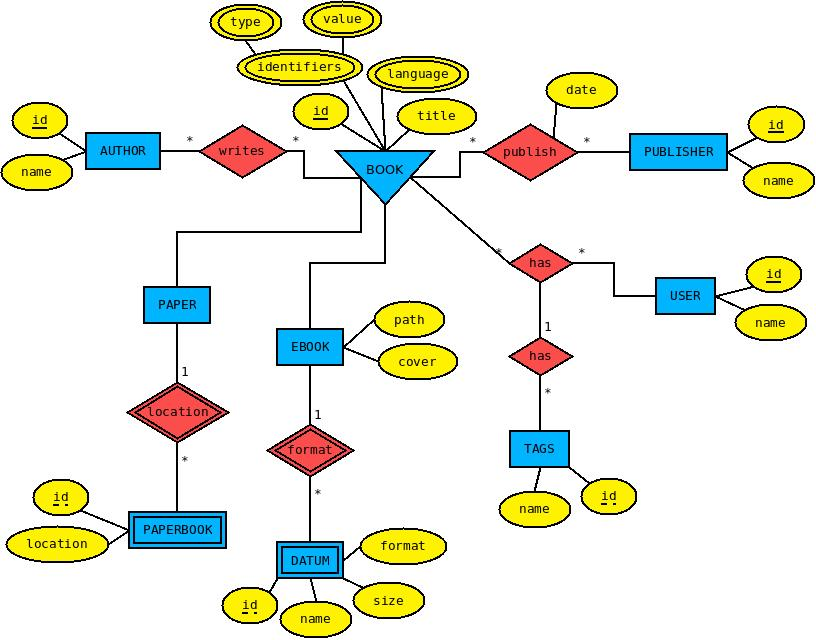
\includegraphics{images/Diagram.jpeg}}
\caption{Διάγραμμα οντοτήτων - συσχετίσεων}
\label{fig:ER:diagram}
\end{center}
\end{figure}
\end{landscape}

\subsection{Λογικός σχεδιασμός}

\subsubsection{Ανάλυση πινάκων}

πρώτος πίνακας

δεύτερος πίνακας κ.λ.π.

πίνακας με τις εξής στήλες (πεδίο, τύπος μεταβλητής, εύρος τιμών, περιγραφή, Πρωτεύον κλειδί(ναι ή όχι), NULL (ναι ή όχι ), ξένο κλειδί (ναί ή όχι).

\subsection{Υλοποίηση}

\phantomsection \label{Βιβλιογραφία}
\addcontentsline{toc}{section}{Βιβλιογραφία}
%\mtcaddchapter[Βιβλιογραφία] % Λόγω του minitoc
\bibliographystyle{plain}
\bibliography{references}

\newpage

\end{document}

